% \documentclass{report}
% 
% \usepackage{fancyhdr}
\usepackage{fourier-orns}
\usepackage{hyperref}%% To refrence links / jumps
\usepackage{chngcntr} %% For some extra counters numberings
\usepackage[a4paper, right = 0.5in, left = 0.5in,top = 1in , bottom = 1in]{geometry}
\usepackage{etoolbox} %% Provides like a language for advanced customization
\usepackage{datetime} %% For dates of course
\usepackage{lastpage} %% provides pages numbers
\usepackage[sc]{titlesec} %% modify titles
\usepackage{enumerate}
\usepackage{cancel}
\usepackage{tikzsymbols}
\usepackage[dvipsnames]{xcolor}
\usepackage{import}
\usepackage{pdfpages} %% include other pdfs
\usepackage{transparent} %% Transparency
\usepackage{xcolor}  %% Colors
\usepackage[many]{tcolorbox}
\usepackage[framemethod=TikZ]{mdframed}
\usepackage{amsmath,amsfonts,amsthm,amssymb,mathtools}
\usepackage{tikz}
\usepackage{bookmark}
\usepackage{graphicx}
\usepackage{mathpazo}

\usepackage{fontawesome5}

\linespread{1.5}


\titleformat{\chapter}[display]   
{\fontfamily{ppl}\selectfont\huge\color{YellowOrange!80!orange}} % Font style and size 
{\raggedleft\color{purple}\fontsize{70}{0pt}\selectfont\thechapter}   
{-1.5cm}    			                          % Space between the chapter number and title
{
	\begin{tikzpicture}[overlay]
		\node[anchor = west,yshift = 0.2cm,xshift = -1cm] {\fontsize{90}{20} $\int_{}^{} $};
		\node[yshift = 4cm, xshift = 17cm]   {\includegraphics[width = 4cm]{preview0}};
	\end{tikzpicture}
\hspace{1cm}\Huge\raggedright\MakeUppercase}

\titleformat{\section}[block]
{
\fontfamily{ppl}\selectfont\huge\color{YellowOrange!80!orange}
}
{
\color{purple}\fontsize{20}{0pt}\selectfont\thesection 
}
{0cm}
{
	\begin{tikzpicture}[overlay]
		\node[anchor = west,yshift = 0.2cm,xshift = -0.4cm, circle = 1pt] {};
	\end{tikzpicture}
}

\titlespacing*{\section}{0pt}{0.7cm}{1.5cm}


\newcommand{\divider}
{
	\begin{center}
	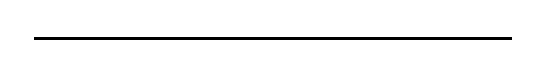
\begin{tikzpicture}
		\draw[thick, black] (0.25*\textwidth, 0) -- (0.75*\textwidth, 0);
		\node[rotate = 360 - 90, xshift = -0.6pt, yshift = 1pt] at (0.25*\textwidth,0){\decotwo};
		\node[rotate = 90, xshift = -0.6pt, yshift = 1pt] at (0.75*\textwidth,0){\decotwo};
	\end{tikzpicture}
	\end{center}
}

\pagestyle{fancy}

\newcommand{\lecday}[1][]
{
    \def\datee{#1}
    \fancyhead[L]{\datee}
}



\newcommand{\signature}
{
	\begin{tikzpicture}[remember picture,overlay]
		\node[fill = YellowOrange!20!white] at ([yshift = 1cm, xshift = -3cm]current page.south east) {\fontsize{10pt}{0pt}{\itshape Kara.$\mathcal{A}$}};
	\end{tikzpicture}
}

\AddToHook{shipout/background}{
  \begin{tikzpicture}[remember picture, overlay]
	  \node[] at ([yshift = 1.5cm,xshift = \textwidth /2 + 0.9cm]current page.south west) {\includegraphics[width = 0.5cm]{preview3}};
	  \node[] at ([yshift = 1.5cm,xshift = - \textwidth /2 - 0.9cm]current page.south east) {\includegraphics[width = 0.5cm]{preview4}};
  \end{tikzpicture}
}



\newtcolorbox[auto counter, number within = section]{remark}[1][]
{
       		title = Remark #1,
		enhanced,
		boxrule = 0pt,
		colback = white,
		breakable,
		arc = 4pt,
		colbacktitle = cyan,
		colback = cyan!5!white,
		segmentation style =
		{
			solid,cyan,thick,
		},
		attach boxed title to top left =
		{
			xshift = 0cm,
		},
		boxed title style =
		{
			boxrule = 0pt,
			sharp corners,
			drop fuzzy shadow = {cyan},
		},
		drop fuzzy shadow = {cyan!80!black},
}

\newtcolorbox[auto counter, number within = section]{theorem}[1][]
{                                      
		title = Theorem \thetcbcounter : #1,
		enhanced, 
		boxrule = 0pt,
		colback = white,
		breakable,
		arc = 4pt,
		colbacktitle = purple,
		colback = purple!5!white,
		segmentation style = 
		{
			solid, purple,thick,
		},
		attach boxed title to top left = 
		{
			xshift = 0cm, 
		},
		boxed title style = 
		{
			boxrule = 0pt,
			sharp corners,
			drop fuzzy shadow = {purple},
		},
		drop fuzzy shadow = {purple!80!black},
}

\newtcolorbox[auto counter, number within = section]{definition}[1][]
{                                      
		title = Definition \thetcbcounter : #1,
		enhanced, 
		boxrule = 0pt,
		colback = white,
		arc = 4pt,
		breakable,
		colbacktitle = YellowOrange!80!black,
		segmentation style = 
		{
			solid, YellowOrange,thick,
		},
		attach boxed title to top left = 
		{
			xshift = 0cm, 
		},
		colback = YellowOrange!5!white,
		boxed title style = 
		{
			boxrule = 0pt,
			sharp corners,
			drop fuzzy shadow = {YellowOrange!80!orange},
		},
		drop fuzzy shadow = {YellowOrange!80!black},
}

\newtcolorbox[auto counter, number within = section]{corollary}[1][]
{                                      
		title = corollary \thetcbcounter : #1,
		enhanced, 
		boxrule = 0pt,
		colback = white,
		arc = 4pt,
		breakable,
		colbacktitle = YellowOrange!80!black,
		segmentation style = 
		{
			solid, YellowOrange,thick,
		},
		attach boxed title to top left = 
		{
			xshift = 0cm, 
		},
		colback = YellowOrange!5!white,
		boxed title style = 
		{
			boxrule = 0pt,
			sharp corners,
			drop fuzzy shadow = {YellowOrange!80!orange},
		},
		drop fuzzy shadow = {YellowOrange!80!black},
}


\newtcolorbox{example}[1][]
{                                      
		title = Example,
		enhanced, 
		boxrule = 0pt,
		colback = white,
		arc = 4pt,
		segmentation style = 
		{
			solid, SpringGreen,thick,
		},
		breakable,
		colback = SpringGreen!5!white,
		colbacktitle = SpringGreen!80!black,
		attach boxed title to top left = 
		{
			xshift = 0cm, 
		},
		boxed title style = 
		{
			boxrule = 0pt,
			sharp corners,
			drop fuzzy shadow = {SpringGreen!80!orange},
		},
		drop fuzzy shadow = {SpringGreen!80!black},
}


\newcommand{\integral}[4]{\int\limits_{#1}^{#2} #4 d#3}
\newcommand{\limit}[3]{\lim\limits_{#1 \rightarrow #2} #3}
\newcommand{\strone}[2]{\left[ \begin{gathered}#1\\ #2\end{gathered} \right] }
\newcommand{\strtwo}[2]{\left\{ \begin{gathered}#1\\ #2\end{gathered} \right\} }
\newcommand{\strthree}[2]{\left\lfloor \begin{gathered}#1\\ #2\end{gathered} \right\rfloor }


\newcommand{\startbf}[1]{\text{\bfseries{#1}}}
\newcommand{\sett}[1]{\left\{ #1 \right\}}
\newcommand{\thesis}[1]{\left( #1 \right)}
\newcommand{\brkt}[1]{\left[ #1 \right]}
\newcommand{\floor}[1]{\left\lfloor #1 \right\rfloor}


\DeclareMathOperator{\img}{im} % Image
\DeclareMathOperator{\Img}{Im} % Image
\DeclareMathOperator{\coker}{coker} % Cokernel
\DeclareMathOperator{\Coker}{Coker} % Cokernel
\DeclareMathOperator{\Ker}{Ker} % Kernel
\DeclareMathOperator{\rank}{rank}
\DeclareMathOperator{\Spec}{Spec} % spectrum
\DeclareMathOperator{\Tr}{Tr} % trace
\DeclareMathOperator{\pr}{pr} % projection
\DeclareMathOperator{\ext}{ext} % extension
\DeclareMathOperator{\pred}{pred} % predecessor
\DeclareMathOperator{\dom}{dom} % domain
\DeclareMathOperator{\ran}{ran} % range
\DeclareMathOperator{\Hom}{Hom} % homomorphism
\DeclareMathOperator{\Mor}{Mor} % morphisms
\DeclareMathOperator{\End}{End} % endomorphism


\newcommand{\lm}{\ensuremath{\lambda}}
\newcommand{\eps}{\ensuremath{\epsilon}}
\newcommand{\veps}{\ensuremath{\varepsilon}}
\newcommand{\al}{\ensuremath{\alpha}}
\newcommand{\bb}{\ensuremath{\beta}}
\newcommand{\cc}{\ensuremath{\gamma}}
\newcommand{\dd}{\ensuremath{\delta}}
\newcommand{\DD}{\ensuremath{\Delta}}
\newcommand{\ff}{\ensuremath{\phi}}
\newcommand{\FF}{\ensuremath{\varphi}}

\newcommand{\RR}{\mathbb{R}}
\newcommand{\RO}{\mathcal{R}}
\newcommand{\EE}{\mathbb{E}}
\newcommand{\CC}{\mathbb{C}}
\newcommand{\RW}{\mathbb{R}^2}
\newcommand{\RT}{\mathbb{R}^3}
\newcommand{\RN}{\mathbb{R}^n}
\newcommand{\DS}{\mathcal{D}}

\newcommand{\KK}{\mathbb{K}}
\newcommand{\KW}{\mathbb{K}^2}
\newcommand{\KT}{\mathbb{K}^3}
\newcommand{\KN}{\mathbb{K}^n}

\newcommand{\NN}{\mathbb{N}}

\newcommand{\PS}{\mathcal{P}}
\newcommand{\AS}{\mathcal{E}}
\newcommand{\FS}{\mathcal{F}}
\newcommand{\LS}{\mathcal{L}}
\newcommand{\MS}{\mathcal{M}}


















\lecday[2025-05-29]

%  \begin{document}
\begin{proof}
It's known that $K^{\bot } $ is a 
\underline{
vector subspace 
} of $H $, of course ( \underline{\textcolor{red}{Algebra 3}} ). Let
us prove that $K^{\bot }$ is closed. \\
let $( x_{n} )_{n \in \NN}  $ be a sequence of $K^{\bot } $, which
converges in $H $ to some $x \in  H $. and let 
us show that we have necessary $x \in  K^{\bot } $, using the 
continuity of the inner product 
\[
  \fbox{
    \textcolor{red}{
      $\left\langle \cdot , \cdot  \right\rangle  $ 
    }
  }
\]
(with respect to it's $1^{st} $ variable). we have for all 
$u \in  K $ : 
\begin{align*}
\left\langle 
  x, u
\right\rangle &= 
\left\langle 
  \lim_{n \to \infty} x_{n}, u
\right\rangle  \\
              &= 
              \lim_{n \to \infty} 
              \left\langle 
                x_{n}, u
              \right\rangle  \\
              &= 
              \lim_{n \to \infty}  0 = 0
\end{align*}
implying that :
\[
\fbox{
$\textcolor{red}{ x \bot  u
  \quad \quad 
\forall u \in K
} 
$
}
\]
Thus consequently, $K^{\bot } $ is closed in $H$.
\\
\underline{
  \large
\textsc{ $K \cap K^{\bot } = \left\{ 0_{H} \right\}$ ? :} 
\warning
}
\\
for all $x \in  K \cap K^{\bot } $, we have 
\[
x \bot x; \quad \text{i.e. }  
\left\langle x, x \right\rangle  = 0 \quad \text{i.e. }  
\| x \| ^2  = 0 \quad \text{i.e. }  
\| x \| = 0  \implies x = 0_{H}
\]
hence $K \cap K^{\bot } \subset \left\{ 0_{H} \right\}$; hence 
\[
K \cap K^{\bot } = \left\{ 0_{H} \right\}
\]
Thus the sum :
\[
  \fbox{
$K + K^{\bot } \quad \quad \text{ \textcolor{blue}{is direct}}$
  }
\]
\underline{
  \large
  \textsc{ $K +  K^{\bot } \overset{?}{=}  H$ :}
\warning
}
\\
Let $x \in  H $ be arbitrary. Consider $u = \pi _{K}(x)  \in  K $. 
By corollary $3 $, we have : 
\[
  \fbox{
    \textcolor{red}{
    $
\left\langle 
  x - \pi _{K}(x) , v 
\right\rangle  = 0 \quad \quad 
\forall  v \in  K$
    }
  }
\]
That is : 
\[
  (x - \pi _{K}(x) )  \in  K^{\bot }
\]
hence : 
\[
x = 
\underbrace{ 
\pi _{K}(x) 
}_{ \in K}  + 
\underbrace{
  (x - \pi _{K}(x) ) 
}_{ \in  K^{\bot }}  \in  K + K^{\bot }
\]
Thus : 
\[
H \subset K + K^{\bot } \subset H
\] 
Hence : 
\[
  \fbox{
    \textcolor{blue}{
$H = K \oplus K^{\bot }$
    }
  }
\]
This 
\underline{completes} the proof.
\end{proof}

\begin{definition}[]
Let $H $ be a Hilbert space, and $K $ be a closed
vector subspace of $H $. Then $K^{\bot } $ is called 
the \underline{orthogonal complement} of $K $ (in $H $).
\end{definition}
\divider
\underline{
  \large
\textsc{Exercise :} 
}
\warning
\normalfont
\\
\lefthand ~
Let $H $ be a \underline{Hilbert} and $K $ be 
a vector subspace of $H $ (not necessary closed). Show that we have : 
\[
  \fbox{
    \textcolor{red}{
     $K^{\bot  \bot } = \overline{K}$ 
    }
  }
\]
\divider
\lefthand ~ The orthogonal \underline{projection} 
on a finite-dimensional vector subspace of a \textcolor{red}{
\underline{Hilbert}} space : 
\\
Let $H $ be a Hilbert space and $F $ be a 
\underline{
finite-dimensional
} vector subspace of $H $, so $F $ is closed in $H $ and 
we can speak about the (orthogonal) projection of a vector 
of $H $ onto $F $ and ask about an expression of it with respect
to the appropriate basis of $F $. \\
In what follows, we will find such an expression relative to 
an orthonormal basis of $F $.\\
Let $\mathcal{B} = (e_1, e_2, \hdots , e_{n})$ 
where $(n = dimF \in  \NN_0)$, be an orthonormal basis 
of $F$ ( $\mathcal{B}  $ exists and it can be formed 
by the \textcolor{red}{Gram-Schmidtz} algorithm for example). 
we have the following proposition : 
\begin{theorem}[]
For every $x \in  H $, we have : 
  \[
      \textcolor{blue}{
    \fbox{
        $\pi _{F}(x) = 
        \sum_{k=1}^{n} 
        \left\langle e_{k}, x \right\rangle e_{k}$ 
      }
    }
  \]
\end{theorem}
\begin{proof}
Let $x \in  H $ be fixed.  \\
since $\pi _{F}(x)  \in  F = \left\langle 
  e_1, e_2, \hdots , e _n 
\right\rangle$, then we can write $\pi _{F}(x)  $ as : 
\[
  \pi _{F}(x) = \sum_{k=1}^{n} 
  \lm_{k} e_{k} \quad (\lm_{k} \in  \CC , k=1, \hdots , n) \quad \quad 
  \quad \quad (1)  
\]
Next, by Corollary $3 $, we have : 
\begin{align*}
  (x-\pi _{F}(x) )  \in  F^{\bot } &=  
  \left\langle 
    e_1, e_2, \hdots , e _n 
  \right\rangle ^{\bot } \\
                                 &= 
              \left\{ e_1, \hdots , e _n  \right\}^{\bot }
\end{align*}
That is : 
\[
\left\langle 
  e_{k}, x-\pi _{F}(x) 
\right\rangle  = 0 \quad \forall k \in  \left\{ 
1, 2, \hdots , n
\right\}
\]
For all $k \in  \left\{ 1, 2, \hdots , n \right\} $, we have :
\begin{align*}
&\iff \left\langle 
  e_{k}, x - \pi _{K}(x) 
\right\rangle  = 0 \\
& \iff 
\left\langle 
  e_{k}, 
  x - \sum_{\ell =1}^{n} 
  \lm_{\ell } e_{\ell }
\right\rangle = 0 \\
& \iff   
\left\langle 
  e_{k}, x
\right\rangle  - 
\sum_{\ell  = 1}^{n}  
\lm_{\ell }
\underbrace{
\left\langle 
  e_{k}, \ell 
\right\rangle 
}_{
    \dd _{k, \ell } = 
    \begin{cases}
      1 \\
      0
    \end{cases}
    \begin{gathered}  
      \text{ if } \ell  = k\\ 
      \text{ else } 
    \end{gathered}
    } 
    \\
&\iff  
\left\langle 
  e_{k}, x
\right\rangle  - \lm_{k} = 0 \\
& \iff 
\lm_{k} = \left\langle 
  e_{k}, x
\right\rangle \quad 
\forall k \in  \left\{ 1, 2, \hdots , n \right\}
\quad \quad \quad (2) \quad 
\end{align*}
By substituting into $(1)$, we get : 
\[
  \textcolor{blue}{
  \fbox{
    $
  \pi _{F}(x)  =
  \sum_{k=1}^{n} 
  \left\langle 
    e_{k}, x
  \right\rangle  e_{k}
  $
  }
  }
\]
As required.

\end{proof}

\begin{corollary}[]
For all $x \in  H $, we have : 
\[
  \textcolor{purple}{
  \fbox{ 
    $\| \pi _{F}(x)  \| ^2 = 
    \sum_{k=1}^{n} 
    \left| 
    \left\langle e_{k}, x \right\rangle 
    \right|^2 $ 
  }
  }
\]
\end{corollary}
\begin{proof}
Since the vectors $\left\langle e_{k}, x \right\rangle e_{k} $ are pairwise
orthogonal, we have by the 
  \textcolor{cyan}{
\underline{
  \textsc{
Pythagorean 
Theorem 
  }
} :
  }
 \begin{align*}
   \| \pi _{F}(x)  \|  &= 
   \| \sum_{k=1}^{n} 
   \left\langle e_{k}, x \right\rangle e_{k}\| ^2  \\
   &=  
   \sum_{k=1}^{n} 
   \underbrace{
   \| 
   \left\langle 
     e_{k},x
   \right\rangle e_{k}
   \| ^2  
   }_{= \left| \left\langle e_{k},x \right\rangle  \right|^2 } 
   = \sum_{k=1}^{n} 
   \left| \left\langle e_{k},x \right\rangle  \right|^2 
 \end{align*}
 as required.
\end{proof}

\begin{center}
  \textcolor{purple}{
  \textsc{
    \underline{
      The Riesz representation Theorem :
    }
  }
  }
\end{center}
\begin{theorem}[(F. Riesz)]
  Let $H$ be a Hilbert space. Then for 
  every $f \in  H' $ there \underline{exists} a 
  \underline{unique} $a \in H $ such that :
  \[
    \textcolor{purple}{
      \fbox{
        $f(x) = \left\langle a,x \right\rangle  \quad 
        \left( \forall x \in  H \right)$
      }
    }
  \]
\end{theorem}
\begin{proof}
Let $f \in  H' $ (i.e. $f $ is contiuous linear form on $H $).
\\
\textsc{
  \large
\underline{
  The existence of $a$   
} : 
\warning
\normalfont
}
\\
If $f = 0_{H'} $, it sufficies to take $a = 0_{H} $. 
Suppose for the sequel that $ f \neq 0_{H'} $. \\
So $Ker(f)$ is a closed (linear) hyperplane of $H $. 
it follows (according to the corollary that $Ker(f) \oplus Ker(f)^{\bot } = H$),
and $dim(Ker(f))^{\bot } = 1$ \footnote {
  A note the teacher wrote, $u, v \in  (ker(f) )^{\bot }$   
  \begin{align*}
    w &= f(v) u - f(u)  v \in Ker(f)^{\bot }  
    \\
    f(w) &=  f(v) f(u)  - f(u) f(v)  = 0
    \\
       &\implies  w \in  Ker(f) \\
       &\implies w \in Ker(f) \cap Ker(f) ^{\bot } = 
    \left\{ 0_{H} \right\} \\
         &\implies 
         w = 0_{H}
  \end{align*}
}, 
let $a_0 \in  (Ker(f) ) ^{\bot } $ such that 
$a_0 \neq 0_{H} $, so : 
\[
  (Ker(f) ) ^{\bot } = 
  \left\langle 
    a_{0}
  \right\rangle 
\]
we have :  
\begin{align*}
  f(a_0)  &= 
  \frac{f(a_0) }{\| a_0 \| ^2 }
  \| a_0 \| ^2  \\
          &= 
          \frac{a_0}{\| a_0 \| ^2 } 
          \left\langle 
            a_0, a_0
          \right\rangle  \\
         &=
         \left\langle 
           \frac{\overline{f(a_0) }}{\| a_0 \| ^2 } 
           a_0, a_0
         \right\rangle  
\end{align*}
set $a := \frac{\overline{f(a_0) }}{\| a_0 \| ^2 }a_0$, so we have :  
\[
  \textcolor{cyan}{
   \fbox{
     $f(a_0) = \left\langle a, a_0 \right\rangle $
   }
  }
\]
now, for all $x \in  H $, for $\lm \in \CC, y \in Ker(f) $, we can write $x $ as :  
\[
x = y + \lm a_0 \quad \quad  \left( 
  \text{ since } H = 
  Ker(f)  \oplus (Ker(f) )^{\bot }= 
  Ker(f) \oplus \left\langle a_0 \right\rangle  
\right)
\]
by inserting $f $ on both sides : 
\begin{align*}
  f(x)  &= f(y + \lm a_0) \\
        &= f(y)  + \lm f(a_0)  \\
        &= \lm \left\langle a, a_0 \right\rangle  \\
        &=
        \underbrace{
        \left\langle a, y \right\rangle 
        }_{=0, \quad y \in  Ker(f), a \in Ker(f)^{\bot } } +  
        \lm
        \left\langle a, a_0 \right\rangle  \\ 
        &= 
        \left\langle a,y  \right\rangle  + 
        \left\langle a, \lm a_0 \right\rangle  
        \\
        &= 
        \left\langle 
          a, y + \lm a_0
        \right\rangle  = \left\langle a,x \right\rangle 
\end{align*}
Hence : 
\[
  \textcolor{blue}{
    \fbox{
      $f(x) = \left\langle a, x \right\rangle \quad \quad (\forall x \in  H)  $
    }
  }
\]
\lefthand ~ As required.
\\
\textsc{
  \large
\underline{
  The uniqueness of $a $
} : 
\warning
\normalfont
}
\\
Let $a,b \in  H $ such that for all $x \in  H $ : 
\[
f(x)  = \left\langle a,x \right\rangle = \left\langle b,x \right\rangle 
\]
thus $\forall x \in  H $ : 
\[
\left\langle a-b, x \right\rangle  = 0
\]
\lefthand ~ Hence $(a-b) \in  H^{\bot } = \left\{ 0_{H} \right\} $, 
thus $a-b = 0_{H}$; thus $a = 0$, hence the uniqueness 
of $a$. This completes the proof. 
\end{proof}
\begin{corollary}[]
  Any \underline{real} \textcolor{red}{Hilbert} space $H $ 
  is \underline{Isometrically isomorphic} to it's \underline{continuous dual} 
  $H'$. 
\end{corollary}
\begin{proof}
Let $H $ be a Hilbert space. Consider : 
\[
\begin{array}{cccc}
      \FF   : &  H  & \longrightarrow & H' \\

           &  a  & \longmapsto     & \FF _{a} \\ 
\end{array}
\]
where $\FF _{a}$ is :
\[
\begin{array}{cccc}
      \FF _{a} : &  H  & \longrightarrow & \RR  \\

           &  x  & \longmapsto     & \left\langle a,x \right\rangle  \\ 
\end{array}
\]
The \textcolor{purple}{
  \textsc{
Riesz Representation Theorem}
  } ensures that $\FF  $ is bijective. Next, 
  it's clear that $\FF  $ is linear and that for all $a \in  H$, we have :  
  \[
  \| \FF (a)  \| _{H'} = 
  \mid \mid \mid  \FF _{a} \mid \mid \mid _{H'} \overset{
    \text{\textcolor{blue}{Cauchy Schwartz}} 
  }{=}  
  \| a \| _{H}
  \]
  Implying that $\FF  $ is an isomorphism isometric of N.V.S
\end{proof}
\begin{center}
  \textsc{
    \textcolor{magenta}{
      \underline{
      \righthand ~ Further Applications of The Riess Representation Theorem ~
      \lefthand
      }
    }
  }
\end{center}
\begin{corollary}[]
  Let $H $ be a Hilbert space and $G $ be a \underline{closed}
  vector subspace of $H$.  \\
  Then, every continuous linear form on $G$ has a unique 
  \textcolor{red}{Hahn-Banach} extension on $H$. Precisely : 
  \[
    \textcolor{purple}{
    \fbox{
      $\forall g \in  G', 
      \quad \exists ! h \in  H', \quad 
      f_{|G} = g \quad \text{ and } \quad 
      \mid \mid \mid  h \mid \mid \mid _{H'} = 
      \mid \mid \mid  g \mid \mid \mid _{G'}$ 
    }
    }
  \]
\end{corollary}
\begin{proof}
  Let $g \in  G'$ and show that $g $ has
  a unique \textcolor{red}{Hahn-Banach} extension in $H $.  
  Since $G$ is closed in $H $ which is a complete space  
  then $G $ is complete; That is, $G $ is \textcolor{purple}{Hilbert}.
  By the 
  \textcolor{purple}{
    \textsc{
  Riesz Representation Theorem 
    }
  }, 
  \[
  \exists ! a \in  G, \quad 
  g(x)  = \left\langle a,x \right\rangle   
  \quad \quad \left( \forall  x \in  G \right)
  \]
  An obvious \textcolor{red}{Hahn-Banach} extension of $g $ 
  on $H $ is $h_1 \in  H'$, given by :  
  \[
  h_1(x) = \left\langle 
    a, x
  \right\rangle   \quad \quad 
  \left( \forall  x \in  H \right)
  \]
  Let us show that this is the unique 
  \textcolor{red}{Hahn-Banach} extension of $g$. 
  Let $h_2 \in  H' $ be another \textcolor{red}{Hahn-Banach} 
  extension of $g $ on $H$. By the 
  \textcolor{purple}{
    \textsc{
  Riesz Representation Theorem 
    }
  } : 
  \[
  \exists ! b \in  H, \quad 
  h_2(x) = \left\langle 
    b,x
  \right\rangle \quad \quad (\forall  x \in  H) 
  \]
  since $h_2 $ extends $g $, we have :
  \begin{align*}
    h_2(x)  &= g(x)  \quad \quad (\forall  x \in  G)  
    \\
    \left\langle b,x \right\rangle  &=
    \left\langle a,x \right\rangle   \quad \quad 
    \left( \forall  x \in  G \right) 
    \\
    \left\langle b-a, x \right\rangle  &= 0  \quad \quad 
    \left( 
      \forall  x \in  G
    \right)
  \end{align*}
  In particular since $a \in G $ :  
  \[
  \left\langle 
    b-a, a
  \right\rangle  = 0
  \]
  thus : 
  \[
    (b-a)  \bot a
  \]
  so, by the 
  \textcolor{cyan}{
    \textsc{
      Pythagorean Theorem
    }
  }, we have : 
  \begin{align*}
    \underbrace{
  \| (b-a) + a  \| ^2  
    }_{= \| b \|^2  } 
  = 
  \| b-a \|  ^2  + 
  \| a \| ^2 
  \end{align*}
  Thus : 
  \[
    \textcolor{magenta}{
      \fbox{
        $\| b-a\|^2  = 
        \| b \|^2  - \| a \|^2$
      }
    }
  \]
  But since $h_2 $ is a \textcolor{red}{Hahn-Banach} extension 
  of $g $, we have : 
  \[
  \mid \mid \mid  h_2 \mid \mid \mid _{H'} = 
  \mid \mid \mid  g \mid \mid \mid _{G'}
  \]
  i.e. 
  \[
  \| b \| = \| a \| 
  \]
  Hence : 
  \[
  \| b-a \| ^2  = 0
  \]
  implying that 
  \[
    b = a
  \]
  Hence $h_2 = h_1$, as required. \\
  This completes the proof
\end{proof}


% \end{document}
